\section{Section: Prelude}

\section{Section Intro}



\begin{frame}[s]{This is the Plan}
  \begin{enumerate}
   \setlength{\itemsep}{1ex plus 1 fil}
    \item \textbf{Introducing Rosenpass,} briefly.
    \item \textbf{The design of Rosenpass} and basics about post-quantum protocols.
    \item \textbf{Hybrid Security} how it can be done and how we do it.
    \item \textbf{ChronoTrigger Attack} and not trusting wall clocks.
    \item \textbf{Protocol proofs} – big old rant!
  \end{enumerate}

  \begin{center}
    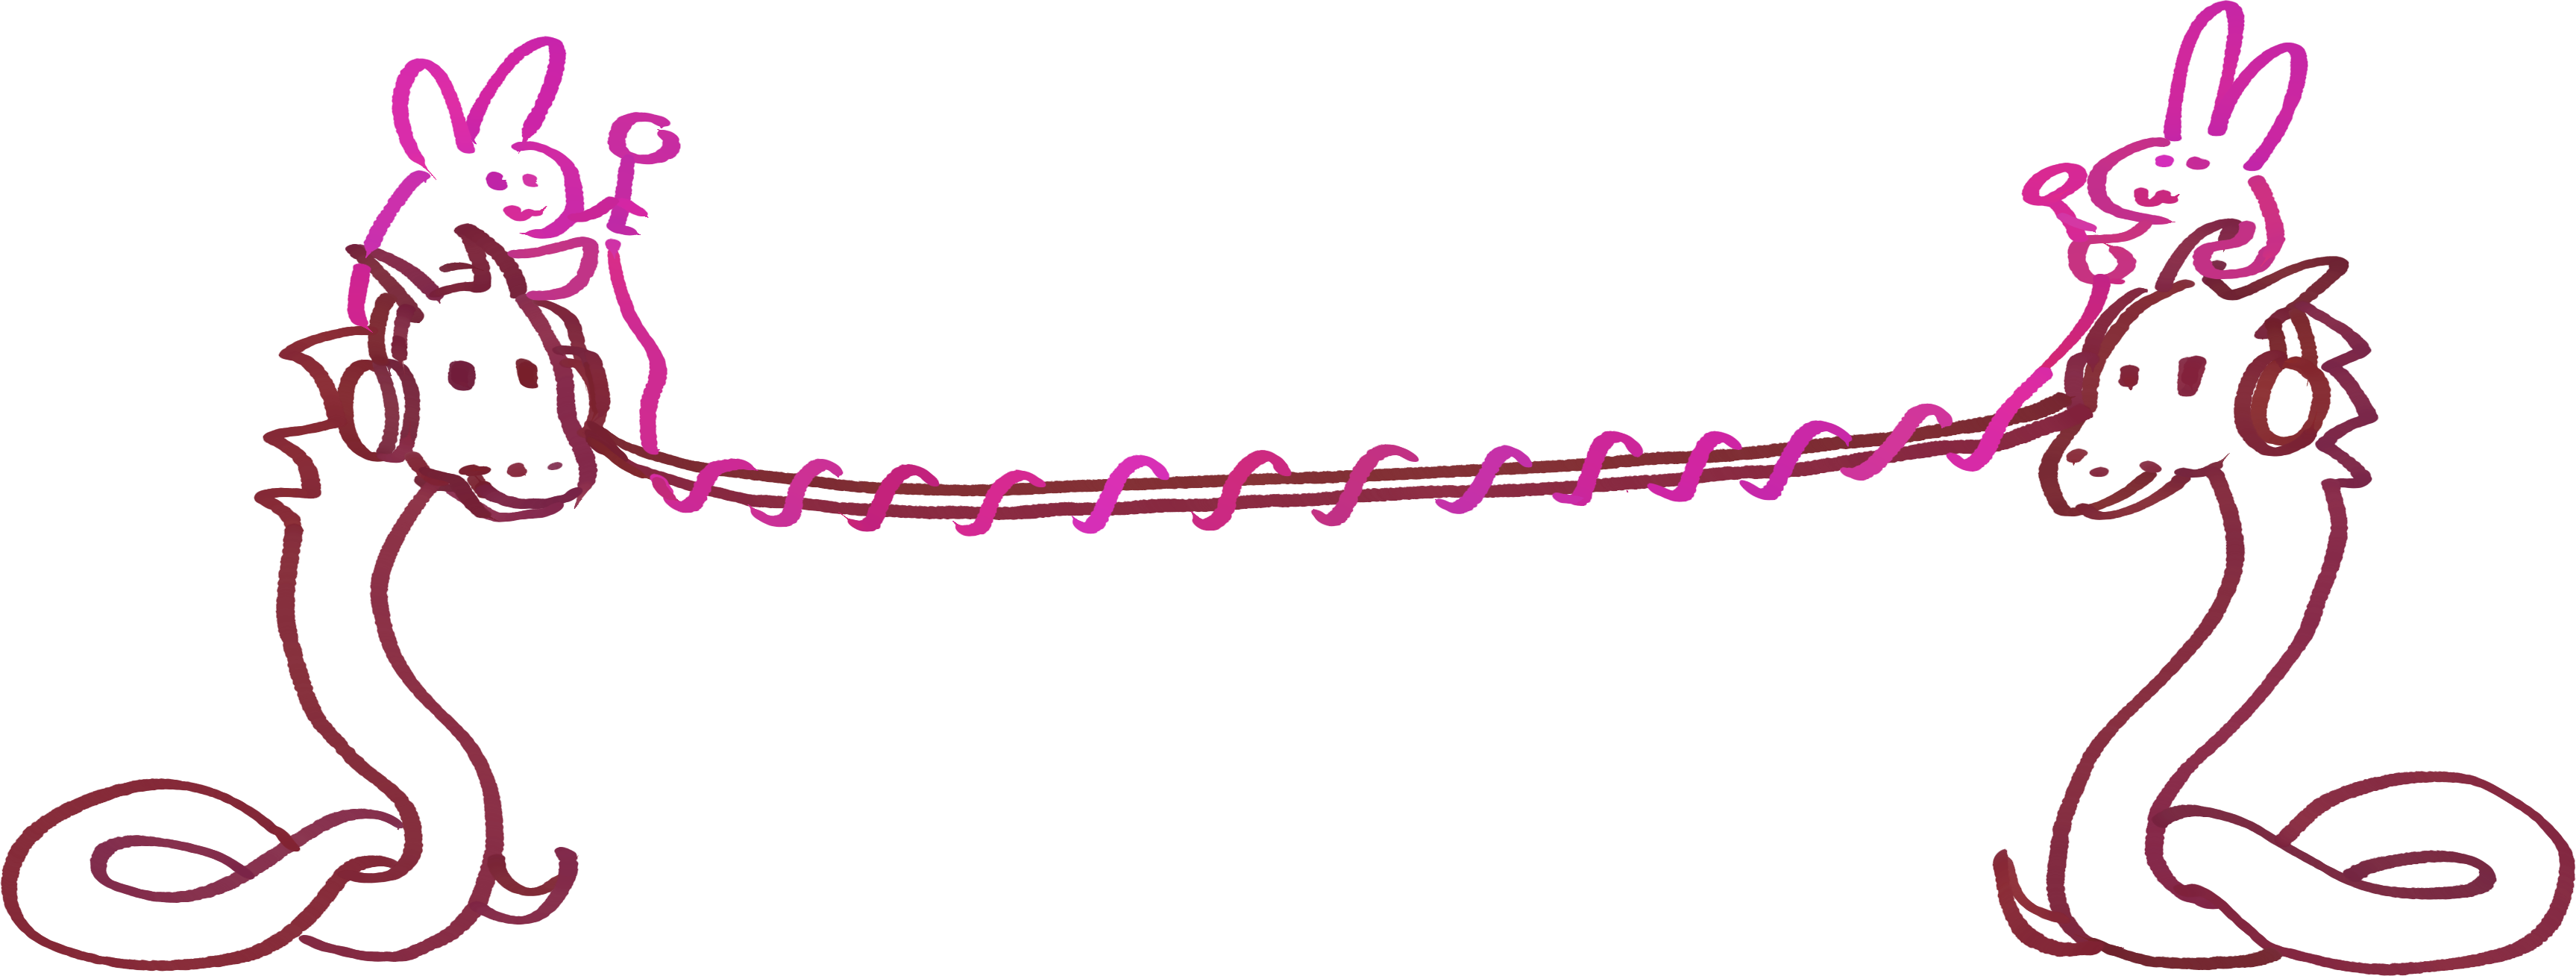
\includegraphics[height=.3\textheight]{graphics/wireguard-and-rp-bunny-rose.png}
  \end{center}
\end{frame}



\begin{frame}{Introducing Rosenpass, briefly}
  \begin{columns}[fullwidth,c]

    \begin{column}{.5\linewidth}
      \begin{itemize}
        \item A post-quantum secure key exchange \textbf{protocol}
          {\small based on the paper Post-Quantum WireGuard\citePqwg}
        \item An open-source Rust \textbf{implementation} of that protocol, already in use
        \item A way to secure WireGuard setups against quantum attacks
        \item A \textbf{post-quantum secure VPN}
        \item A governance \textbf{organization} to facilitate development, maintenance and adoption of said protocol
        %\item A translation research organization
      \end{itemize}
      \vspace{2em}
      \textbf{\href{https://rosenpass.eu}{rosenpass.eu}}
    \end{column}%

    \begin{column}{.5\linewidth}
      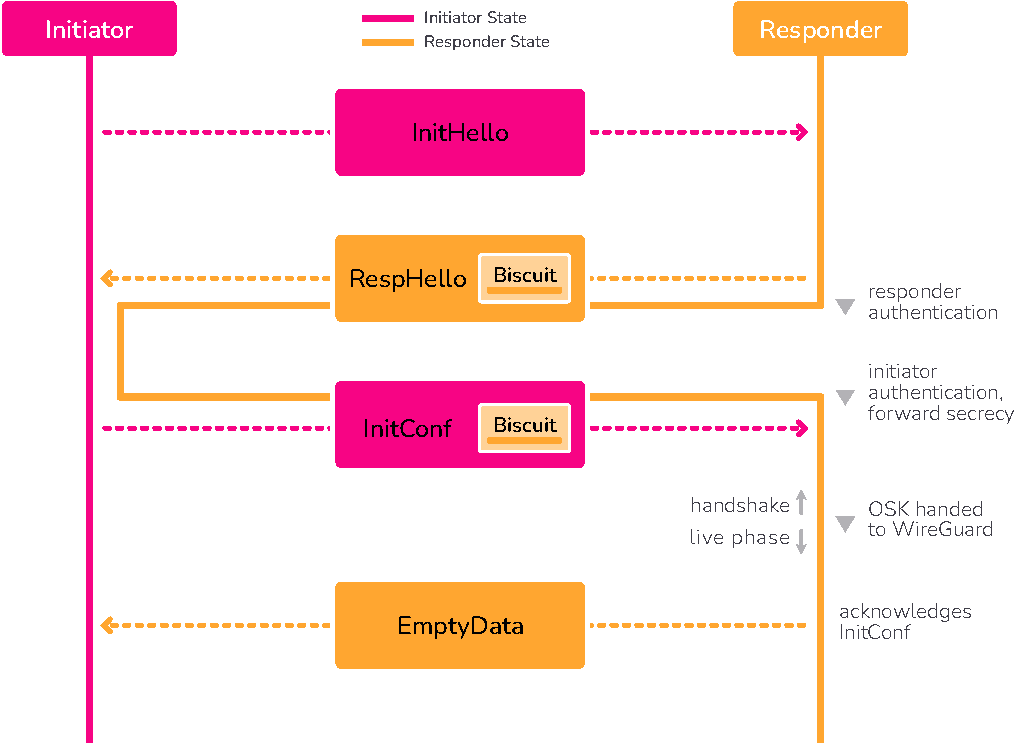
\includegraphics[ width=\linewidth]{graphics/rosenpass-wp-key-exchange-protocol-rgb.pdf}
    \end{column}

  \end{columns}
\end{frame}
